\section{Methods}

The project will be divided into two main parts: the implementation of the \acrshort{simple} algorithm and the analysis of the velocity field around a 2D geometry.

\subsection{SIMPLE algorithm}

The \acrshort{simple} algorithm will be implemented starting from the same codebase used for the first assignment, which already contains the \acrshort{scgs} algorithm.
The codebase has been written in \texttt{C} and from the beginning has been designed to be modular and easily extendable with new algorithms and features.

The \acrshort{simple} algorithm will be implemented following the guidelines provided in the course notes and at first will be able to just solve the steady state Navier-Stokes equations for a 2D problem ($u$, $v$, and $p$).

The code will be tested using the same test cases used for the \acrshort{scgs} algorithm, and the results will be compared with the ones obtained with the \acrshort{scgs} algorithm.

\subsection{Velocity field analysis}

The velocity field analysis will be performed using the same codebase and the \acrshort{simple} algorithm.

We will use our code to answer the question of interest to us: \emph{Investigating the distribution of flow velocity around a pillar during windy conditions to enhance personal comfort by determining the optimal position that reduces wind exposure.}

The problem will make use of multiple simplifying assumptions, so to be simple enough to be modeled within our 2D solver, but at the same time complex enough to analyze a real world problem.

As a real world scenario where our analysis could be useful, we can think of a person waiting for a bus or a train on a windy day at a station with only a pillar that can be used as a shield.
At the end of the project, we will be able to provide a map of the flow velocity distribution around the pillar, based on the wind speed and direction.
Eventually, multiple simple geometry will be tested (e.g. a circular pillar, a square pillar, etc.) and the results will be compared.

\begin{figure}[H]
    \centering
    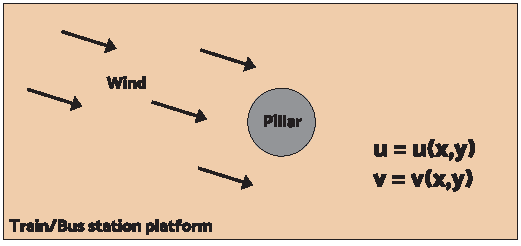
\includegraphics[width=0.8\textwidth]{pdf/problem_drawing}
    \caption{Problem drawing and real world scenario.}
    \label{fig:problem_drawing}
\end{figure}
